\documentclass[12pt, a4paper]{article}

% ---------------------------------------------------------------
% TU IoST §10.6 COMPLIANCE
% ---------------------------------------------------------------

% ---------------------------------------------------------------
% Packages
% ---------------------------------------------------------------

% --- Core Packages ---
\usepackage[table]{xcolor}
\usepackage[top=1in, bottom=1in, left=1.5in, right=1in]{geometry}
\usepackage{mathptmx}            
\usepackage[T1]{fontenc}
\usepackage{setspace}
\onehalfspacing

% --- Layout & Typography ---
\usepackage{titlesec}
\usepackage{tocloft}
\usepackage{titletoc}
\usepackage{fancyhdr}
\usepackage{float}
\usepackage{enumitem}
\usepackage{multirow}
\usepackage{url}
\usepackage{booktabs}
\usepackage{array}

% --- Math & Graphics ---
\usepackage{amsmath}
\usepackage{amssymb}
\usepackage{graphicx}
\usepackage{tikz}
\usetikzlibrary{shapes.geometric, arrows.meta, positioning, fit, backgrounds, calc}

% --- Bibliography (Fixed) ---
\usepackage[style=authoryear, backend=biber, sorting=ynt, maxbibnames=99]{biblatex}
\addbibresource{references.bib}

% --- Hyperref (should be near the end) ---
\usepackage[hidelinks]{hyperref}

% --- Additional packages ---
\usepackage{csquotes}
\usepackage{xurl}

% ---------------------------------------------------------------
% Custom Settings
% ---------------------------------------------------------------
\definecolor{ganttblue}{RGB}{100, 149, 237}
\numberwithin{equation}{section}

\setlength{\parindent}{0pt}
\setlength{\parskip}{6pt}

% Widow/Orphan control
\clubpenalty=10000
\widowpenalty=10000
\displaywidowpenalty=10000

% ---------------------------------------------------------------
% Headings (TU IoST Style)
% ---------------------------------------------------------------
\titleformat{\section}
  {\bfseries\fontsize{14}{17}\selectfont}{\thesection.}{0.5em}{}
\titleformat{name=\section,numberless}
  {\bfseries\fontsize{14}{17}\selectfont}{}{0pt}{}

\titleformat{\subsection}
  {\bfseries\fontsize{12}{15}\selectfont}{\thesubsection}{1em}{}
\titleformat{\subsubsection}
  {\bfseries\fontsize{12}{15}\selectfont}{\thesubsubsection}{1em}{}

\titlespacing*{\section}{0pt}{14pt}{8pt}
\titlespacing*{\subsection}{0pt}{12pt}{6pt}
\titlespacing*{\subsubsection}{0pt}{10pt}{4pt}

% ---------------------------------------------------------------
% TOC Formatting
% ---------------------------------------------------------------
\renewcommand{\cftsecfont}{\bfseries\fontsize{14}{17}\selectfont}
\renewcommand{\cftsecpagefont}{\bfseries\fontsize{14}{17}\selectfont}
\renewcommand{\cftsecleader}{\cftdotfill{\cftdotsep}}
\setlength{\cftsecindent}{0pt}
\setlength{\cftsecnumwidth}{2.5em}
\setlength{\cftbeforesecskip}{12pt}

\renewcommand{\cftsubsecfont}{\fontsize{12}{15}\selectfont}
\renewcommand{\cftsubsecpagefont}{\fontsize{12}{15}\selectfont}
\setlength{\cftsubsecindent}{2.5em}
\setlength{\cftsubsecnumwidth}{3em}

\renewcommand{\cftsubsubsecfont}{\fontsize{12}{15}\selectfont}
\renewcommand{\cftsubsubsecpagefont}{\fontsize{12}{15}\selectfont}
\setlength{\cftsubsubsecindent}{5.5em}
\setlength{\cftsubsubsecnumwidth}{3.5em}

\setcounter{tocdepth}{3}
\setcounter{secnumdepth}{3}

% ---------------------------------------------------------------
% Header/Footer
% ---------------------------------------------------------------
\fancyhf{}
\fancyfoot[C]{\fontsize{10}{12}\selectfont\thepage}
\renewcommand{\headrulewidth}{0pt}
\pagestyle{fancy}

% ---------------------------------------------------------------
% List of Figures/Tables
% ---------------------------------------------------------------
\renewcommand{\cftfigfont}{\fontsize{12}{15}\selectfont}
\renewcommand{\cftfigpagefont}{\fontsize{12}{15}\selectfont}
\renewcommand{\cfttabfont}{\fontsize{12}{15}\selectfont}
\renewcommand{\cfttabpagefont}{\fontsize{12}{15}\selectfont}
\setlength{\cftbeforefigskip}{4pt}
\setlength{\cftbeforetabskip}{4pt}

\renewcommand{\listfigurename}{List of Figures}
\renewcommand{\listtablename}{List of Tables}

\begin{document}
% ==================== TITLE PAGE ====================
\begin{titlepage}
\thispagestyle{empty}
\begin{center}
    \vspace*{1cm}
    {\fontsize{18}{22}\selectfont\bfseries
    Graph Neural Networks for the Classification and Lead Identification
    of EGFR Inhibitors in Non-Small Cell Lung Cancer
    }\\[1.5cm]
    
\includegraphics[width=2in,height=2in,keepaspectratio]{logo-eps-converted-to.pdf}\\[1.5cm]
    {\fontsize{14}{18}\selectfont\bfseries
    A Thesis Proposal Submitted to the\\
    Department of Mathematics\\
    School of Mathematical Sciences, Balkhu\\
    Tribhuvan University\\
    for Approval
    }\\[2cm]
    {\fontsize{14}{18}\selectfont By}\\[0.5em]
    {\fontsize{14}{18}\selectfont\bfseries
    Krishna Gaire\\
    Symbol No.: 7916015\\
    T.U. Registration No.: 5-3-28-49-2022
    }\\[2cm]
    {\fontsize{14}{18}\selectfont\bfseries MAY, 2026}
\end{center}
\end{titlepage}

% ==================== FRONT MATTER ====================
\pagenumbering{roman}
\setcounter{page}{1}

% ==================== TABLE OF CONTENTS ====================
{\singlespacing
\tableofcontents
}
\newpage

% ==================== LIST OF FIGURES ====================
{\singlespacing
\listoffigures
}
\newpage

% ==================== LIST OF TABLES ====================
{\singlespacing
\listoftables
}
\newpage

% ==================== LIST OF ABBREVIATIONS ====================
\section*{List of Abbreviations and Acronyms}
\addcontentsline{toc}{section}{List of Abbreviations and Acronyms}
{\singlespacing
\begin{tabbing}
\hspace{4.5cm} \= \kill
\textbf{AUC-ROC}      \> Area Under the Receiver Operating Characteristic Curve \\
\textbf{CADD}         \> Computer-Aided Drug Design \\
\textbf{ChEMBL}       \> Chemistry European Molecular Biology Laboratory Database \\
\textbf{ECFP}         \> Extended Connectivity Fingerprint \\
\textbf{EGFR}         \> Epidermal Growth Factor Receptor \\
\textbf{F1}           \> F1-Score (Harmonic Mean of Precision and Recall) \\
\textbf{GAT}          \> Graph Attention Network \\
\textbf{GCN}          \> Graph Convolutional Network \\
\textbf{GNN}          \> Graph Neural Network \\
\textbf{GNNExplainer} \> Graph Neural Network Explainer \\
\textbf{IC$_{50}$}    \> Half-Maximal Inhibitory Concentration \\
\textbf{IoST}         \> Institute of Science and Technology \\
\textbf{MCC}          \> Matthews Correlation Coefficient \\
\textbf{MPNN}         \> Message Passing Neural Network \\
\textbf{NSCLC}        \> Non-Small Cell Lung Cancer \\
\textbf{PAINS}        \> Pan-Assay Interference Compounds \\
\textbf{pIC$_{50}$}   \> Negative Logarithm of IC$_{50}$ \\
\textbf{PyG}          \> PyTorch Geometric \\
\textbf{QSAR}         \> Quantitative Structure--Activity Relationship \\
\textbf{RF}           \> Random Forest \\
\textbf{SHAP}         \> SHapley Additive exPlanations \\
\textbf{SMILES}       \> Simplified Molecular Input Line Entry System \\
\textbf{TKI}          \> Tyrosine Kinase Inhibitor \\
\textbf{TU}           \> Tribhuvan University \\
\textbf{XAI}          \> Explainable Artificial Intelligence \\
\textbf{XGBoost}      \> Extreme Gradient Boosting \\
\end{tabbing}
}
\newpage

% ==================== MAIN TEXT ====================
% §10.6: 1.5 line spacing applies from here onwards in body text
\pagenumbering{arabic}
\setcounter{page}{1}

% ==================== CHAPTER 1 ====================
\section{Introduction}

\subsection{Background}

Cancer remains one of the most significant public health challenges of the twenty-first century. Among all cancer types, lung cancer is the leading cause of cancer-related mortality worldwide. According to GLOBOCAN 2022, lung cancer accounted for nearly 1.8 million deaths globally in 2022 \cite{siegel2023}. Non-Small Cell Lung Cancer (NSCLC) represents approximately 85\% of all lung cancer cases. In Nepal and across South and East Asia, the burden is particularly severe, with most patients diagnosed at advanced stages and limited access to targeted therapies.
\parencite{siegel2023}

A major clinically validated therapeutic target in NSCLC is the Epidermal Growth Factor Receptor (EGFR). EGFR is a transmembrane receptor tyrosine kinase that, under normal conditions, regulates cell growth, differentiation, and survival. Somatic mutations in the EGFR kinase domain cause constitutive activation of the receptor, leading to uncontrolled cell proliferation and tumour development. The most common sensitizing mutations are exon 19 in-frame deletions (Ex19del, $\approx$45\% of cases) and the L858R substitution in exon 21 ($\approx$40\% of cases). These mutations are found in 10--15\% of Caucasian NSCLC patients and up to 40--50\% of Asian patients, underscoring the high relevance of EGFR-targeted therapy in the Nepali and broader Asian context \cite{siegel2023}.

Three generations of EGFR tyrosine kinase inhibitors (TKIs) have been developed to block this aberrant signalling. While these inhibitors have significantly improved patient outcomes, acquired resistance remains a major clinical challenge. Resistance to the current standard third-generation TKI, osimertinib, frequently occurs within 9--18 months, often through the C797S mutation, resulting in triple-mutant EGFR (e.g., Ex19del/T790M/C797S) that is resistant to all approved EGFR TKIs \cite{malik2025}. This creates an urgent unmet need for novel EGFR inhibitor chemotypes.

Traditional drug discovery is slow, costly, and resource-intensive. Computational methods, particularly machine learning, have emerged as powerful tools to accelerate the process by enabling large-scale \textit{in silico} screening of chemical libraries \cite{schneider2020}. Graph Neural Networks (GNNs) are especially well-suited for this task because molecules can be naturally represented as graphs, with atoms as nodes and chemical bonds as edges. GNNs can learn rich, task-specific molecular representations directly from structure without depending on hand-crafted descriptors \cite{hu2020}.

Despite promising progress, gaps remain in the application of GNNs for EGFR inhibitor discovery. Most current models function as black-box systems and focus primarily on classification, offering limited interpretability regarding the structural features responsible for activity \cite{jimenez2020}. Moreover, few studies have extended high-performing GNN models beyond classification to practical lead identification through virtual screening of large external compound libraries \cite{sun2021}.

This thesis directly addresses these limitations. It focuses on the development, optimization, and benchmarking of Graph Neural Networks (specifically GCN and GAT models) for the accurate classification of EGFR inhibitors. The best-performing model will then be applied for lead identification through virtual screening of unseen ChEMBL compounds to discover and prioritize potential novel EGFR inhibitors for Non-Small Cell Lung Cancer.

\subsection{Objectives}

\subsubsection{General Objective}
Develop Graph Neural Network for the binary classification of EGFR inhibitors, evaluate performance against traditional machine learning baselines (Random Forest and XGBoost), and apply GNN model for virtual screening of unseen ChEMBL compounds to identify and prioritize potential lead compounds.

\subsubsection{Specific Objectives}
\begin{enumerate}
    \item Develop and train Graph Neural Network models for binary classification of EGFR inhibitor activity (active vs. inactive).
    \item Benchmark the performance of the developed GNN models against strong traditional machine learning baselines Random Forest and XGBoost.
    \item Apply the GNN model for virtual screening on unseen compounds from the ChEMBL database (target CHEMBL203) to identify, prioritize, and rank potential lead compounds for further experimental validation.
\end{enumerate}

\subsection{Rationale}

\textbf{Clinical need:} EGFR resistance mutations (T790M, C797S) are a major unsolved problem in NSCLC treatment. No approved drug overcomes the triple mutant (Ex19del/T790M/C797S). Computational tools are urgently needed to accelerate the discovery of next-generation EGFR inhibitors \cite{rotow2023}.

\textbf{Scientific need:} GNNs have demonstrated competitive performance for molecular activity prediction, yet their black-box nature limits utility to medicinal chemists. Explainability tools exist but have not been systematically applied to EGFR inhibitor prediction. Furthermore, no study has applied a trained EGFR GNN model to downstream virtual screening of unseen ChEMBL compounds. These represent the clear literature gaps this thesis addresses \cite{jimenez2020, jiang2021}.

\textbf{Practical need:} This study uses freely available public data (ChEMBL) and open-source tools (PyTorch Geometric, RDKit, SHAP). It is computationally feasible within the one-month research timeline and is appropriate in scope for a master's level research project at Tribhuvan University.

\subsection{Research Questions}

\begin{enumerate}
    \item What extent does Graph Neural Networks outperform or match conventional machine learning models (Random Forest and XGBoost) in the binary classification of EGFR inhibitors (active vs. inactive)?
    \item How effectively does the best-performing GNN model perform in virtual screening of unseen compounds from the ChEMBL database (target CHEMBL203) for the identification, prioritization, and ranking of potential lead compounds?
\end{enumerate}

\subsection{Significance of the Study}

This study makes three contributions. First, it provides a rigorous comparative analysis of GNN versus traditional ML approaches for EGFR inhibitor classification using multiple data splitting strategies, addressing a gap in evaluation methodology. Second, it delivers the first systematic GNN explainability analysis focused specifically on EGFR inhibitors, connecting model predictions to actionable chemical insights for lead optimization. Third, by applying the best model to virtual screening of unseen ChEMBL compounds, this study produces a ranked list of potential novel EGFR inhibitor candidates for future experimental investigation \cite{walters2020}.

\subsection{Limitations}

\begin{itemize}
    \item \textbf{Computational study only:} No experimental (in vitro or in vivo) validation is performed.
    \item \textbf{Data quality dependence:} Model performance depends on the quality and completeness of ChEMBL bioactivity data, which may contain experimental noise from varying assay conditions.
    \item \textbf{2D molecular graphs:} Three-dimensional conformational effects and protein--ligand binding geometry are not captured.
    \item \textbf{Binary classification scope:} The model predicts active or inactive labels only. Regression of precise binding affinity (pIC$_{50}$) values is beyond the scope of this study.
    \item \textbf{Single primary target:} The study focuses on human wild-type EGFR (ChEMBL203). Generalisation to mutant forms (T790M, C797S) is left as future work.
    \item \textbf{Virtual screening without experimental validation:} Compounds prioritized by virtual screening are computational predictions only.
\end{itemize}

\newpage

% ==================== CHAPTER 2: LITERATURE REVIEW ====================
\section{Literature Review}

\subsection{EGFR as a Therapeutic Target in NSCLC}

The Epidermal Growth Factor Receptor (EGFR), also known as ErbB1 or HER1, belongs to the ErbB family of receptor tyrosine kinases. It consists of an extracellular ligand-binding domain, a single transmembrane domain, and an intracellular kinase domain. Under normal conditions, EGFR is activated by binding of growth factors such as EGF and TGF-$\alpha$, leading to receptor dimerization, autophosphorylation, and activation of downstream signaling cascades including RAS--RAF--MEK--ERK and PI3K--AKT--mTOR, which regulate cell proliferation and survival \cite{siegel2023}.

In NSCLC, somatic mutations in the EGFR kinase domain disrupt this regulation. The most common sensitizing mutations are in-frame deletions in exon 19 (Ex19del, $\approx$45\%) and the L858R point mutation in exon 21 ($\approx$40\%), which together account for 85--90\% of EGFR-mutant NSCLC cases. EGFR mutations are found in 10--15\% of Caucasian and up to 40--50\% of Asian NSCLC patients \cite{siegel2023}. This disproportionately high prevalence in Asian populations makes EGFR-targeted therapy particularly relevant to the Nepali clinical context, where late-stage diagnosis and limited therapeutic access remain persistent challenges.

\subsection{Generations of EGFR TKIs and Resistance Mechanisms}

The clinical development of EGFR TKIs has progressed through three generations, each engineered to overcome the specific resistance mechanism that defeated the previous one \cite{rotow2023}.

\textbf{First-generation TKIs} (gefitinib, erlotinib) are reversible competitive inhibitors of the EGFR ATP-binding pocket. Although they demonstrated remarkable clinical efficacy in sensitizing-mutation carriers, resistance emerged in virtually all patients within 9--13 months, most commonly through the T790M ``gatekeeper'' substitution at position 790, which sterically hinders drug binding and simultaneously increases ATP affinity \cite{leonetti2019}.

\textbf{Second-generation TKIs} (afatinib, dacomitinib) are irreversible pan-ErbB inhibitors that covalently bind to Cys797. Although effective in T790M-harbouring cell lines, dose-limiting wild-type EGFR toxicity restricted their clinical utility, and T790M resistance still emerged in most patients \cite{leonetti2019}.

\textbf{Third-generation TKIs} (osimertinib, rociletinib) were specifically designed to target T790M-mutant EGFR while sparing wild-type receptor. Osimertinib is now the standard first-line treatment for EGFR-mutant NSCLC and has demonstrated superior progression-free survival compared to first-generation agents. However, acquired resistance develops through several mechanisms, most importantly the C797S substitution at the covalent binding site. The triple-mutant combination (Ex19del/T790M/C797S or L858R/T790M/C797S) confers resistance to all currently approved EGFR TKIs, representing a critical unmet clinical need \cite{rotow2023, malik2025}.

\subsection{Bioactivity Data and the ChEMBL Database}

The ChEMBL database (version 33), maintained by EMBL-EBI, is the most widely used public bioactivity resource in cheminformatics, containing IC$_{50}$, K$_i$, and other measurements for millions of small molecules tested against thousands of biological targets \cite{mendez2019}. For this study, the relevant target is human EGFR under ChEMBL identifier CHEMBL203.

A central challenge when using ChEMBL data is experimental heterogeneity: measurements are sourced from many laboratories using different assay protocols, introducing noise and systematic biases. Rigorous data curation --- including conversion to the pIC$_{50}$ scale ($-\log_{10}$[IC$_{50}$]), removal of ambiguous or censored entries, and aggregation of duplicate measurements using geometric means --- is therefore essential before any modelling step \cite{wu2018}. The pIC$_{50}$ scale is preferred because it compresses the wide numerical range of IC$_{50}$ values and more closely approximates a normal distribution, which is better suited to both statistical analysis and machine learning.

\subsection{Molecular Fingerprints and Traditional Machine Learning Baselines}

Before the advent of GNNs, fixed-length molecular fingerprints combined with classical classifiers dominated computational drug discovery. Morgan fingerprints (also called Extended Connectivity Fingerprints, ECFP) encode the circular atomic neighbourhood up to a specified radius as a binary bit vector, capturing local chemical environments efficiently \cite{rogers2010}. ECFP4 (radius = 2, 2048 bits) computed by RDKit remains the most widely used fingerprint in activity prediction benchmarks.

Random Forest (RF) and XGBoost are the two most prominent classifiers applied to fingerprint vectors in cheminformatics. RF builds an ensemble of decision trees on random data subsets and averages predictions, offering robustness to overfitting and native feature importance scores \cite{jiang2021}. XGBoost builds trees sequentially through gradient boosting, consistently achieving state-of-the-art performance on tabular data and remaining a standard strong baseline in molecular property prediction \cite{jiang2021}. The fundamental limitation shared by both approaches is that the molecular representation is hand-engineered and fixed, potentially losing information about global topological features and long-range atomic interactions.

\subsection{Graph Neural Networks for Molecular Property Prediction}

Graph Neural Networks (GNNs) represent a paradigm shift in molecular machine learning by operating directly on the molecular graph structure rather than on a pre-computed fingerprint. The core operation is \textit{message passing}: in each layer, every atom (node) aggregates feature information from its bonded neighbours, producing an updated embedding that encodes an increasingly wide chemical context with each successive layer. After $L$ layers, a global readout function (sum or mean pooling) aggregates all atom-level embeddings into a fixed-size molecule-level vector for downstream classification or regression \cite{gilmer2017}.

The Graph Convolutional Network (GCN) of Kipf and Welling \cite{kipf2017} is the simplest and most widely used GNN architecture for molecular tasks. Each layer computes a degree-normalised weighted average of neighbour features, providing computational efficiency while capturing local chemical context. The Graph Attention Network (GAT) \cite{velickovic2018} extends GCN by replacing fixed normalisation coefficients with learnable attention weights computed from paired node features. This allows the model to selectively attend to the most chemically relevant neighbouring atoms and provides an additional source of molecular interpretability through the attention map.

Comparative benchmarks across multiple molecular datasets consistently show that GNNs match or outperform fingerprint-based methods, particularly when molecular diversity is high and when the structural patterns governing activity are complex \cite{jiang2021}. A large-scale pre-training study on 2 million unlabelled molecules demonstrated that GNNs can learn transferable chemical representations that substantially improve performance on downstream tasks with limited labelled data \cite{hu2020}.

\subsection{GNN Models for EGFR Inhibitor Prediction}

The most directly relevant prior work is DeepEGFR \cite{malik2025}, a GAT-based deep learning model trained on ChEMBL EGFR bioactivity data. DeepEGFR achieved high classification accuracy in distinguishing active from inactive EGFR inhibitors and represented a significant advance over earlier fingerprint-based models. However, DeepEGFR has three important limitations that this thesis directly addresses: (1) it provides no explanation of why specific molecules are predicted as active; (2) it evaluates model performance only with random splitting, which overestimates real-world generalisation; and (3) it does not proceed to apply the trained model for virtual screening of unseen chemical space to identify novel lead compounds.

An earlier influential study by Jiang et al.\ \cite{jiang2021} systematically compared descriptor-based and graph-based models across multiple molecular property prediction datasets and found that GNNs offered advantages particularly for structurally diverse datasets, establishing the methodological foundation for GNN-based molecular activity prediction.

\subsection{Explainability in GNN-Based Drug Discovery}

The explainability gap in deep learning for drug discovery has been extensively reviewed by Jim\'{e}nez-Luna et al.\ \cite{jimenez2020}, who identified the inability to explain GNN predictions in chemically interpretable terms as the primary barrier to adoption by medicinal chemists. Two complementary methods address this gap.

\textbf{GNNExplainer} \cite{ying2019} is a post-hoc, instance-level explainability method that, given a trained GNN and a specific molecule, identifies the minimal subgraph maximising the mutual information between the masked graph and the model's prediction. The output is atom-level and bond-level importance scores, directly visualisable as colour-highlighted molecular graphs. For EGFR inhibitor prediction, this reveals which specific ring systems, hydrogen bond donors, or halogen substituents the model associates with inhibitory activity.

\textbf{SHAP} (SHapley Additive exPlanations) \cite{lundberg2017} provides complementary dataset-level global feature importance by quantifying, across all molecules in the dataset, which atomic properties (aromaticity, hybridization, formal charge, ring membership) most consistently drive predictions of EGFR inhibitory activity. The combination of GNNExplainer (instance-level) and SHAP (dataset-level) provides a complete picture of what the model has learned, transforming a black-box GNN into a chemically interpretable predictive tool.

Despite these tools being available, no published study has systematically applied GNNExplainer or SHAP specifically to EGFR inhibitor predictions. This constitutes the primary scientific literature gap that this thesis targets \cite{jimenez2020}.

\subsection{Virtual Screening with Machine Learning}

Virtual screening is the computational process of evaluating large chemical libraries to prioritize compounds most likely to be active against a biological target, before any laboratory experiments are performed. Machine learning-based ligand virtual screening has emerged as a cost-effective and scalable alternative to physics-based docking for large compound libraries \cite{walters2020, sun2021}.

In a ligand-based ML virtual screening workflow, a model trained on known active and inactive compounds is applied to an unseen external library. Compounds are ranked by predicted activity probability, and top-ranked hits are selected for experimental validation. Applicability Domain (AD) analysis, typically implemented through Tanimoto similarity filtering against the training set, is applied to ensure that predictions are made only for compounds that are structurally similar enough to the training data to warrant confidence \cite{tropsha2020}.

Recent studies have demonstrated the utility of GNN-based virtual screening in identifying novel active scaffolds distinct from known drugs. Stokes et al.\ \cite{stokes2020} applied a GNN trained on antibiotic growth-inhibition data to screen over 100 million compounds and identified halicin, a structurally novel antibiotic with broad-spectrum activity, as a top-ranked hit. This landmark study established proof-of-concept for GNN-driven lead discovery from large chemical databases. Despite this precedent, published EGFR GNN models have focused exclusively on classification accuracy and have not applied trained models for prospective screening of new ChEMBL compounds --- the practical gap this thesis addresses.

\subsection{Summary and Research Gap}

The literature review reveals that while GNNs have been successfully applied to EGFR inhibitor classification \cite{malik2025} and explainability methods have been developed for GNNs \cite{jimenez2020, ying2019}, no published study has integrated all three components --- GNN-based EGFR classification, molecular-level explainability analysis, and virtual screening of unseen compounds --- into a single unified pipeline. This thesis fills all three gaps simultaneously, advancing both the scientific understanding of structural determinants of EGFR inhibitory activity and the practical goal of identifying novel lead compounds for drug-resistant NSCLC.

\newpage

% ==================== CHAPTER 3: MATERIALS AND METHODS ====================
\section{Materials and Methods}

\subsection{Overview of the Computational Pipeline}

This study follows a four-phase computational pipeline: (1) Data Acquisition and Curation, (2) Molecular Graph Construction, (3) Model Development \& Benchmarking, and (4) Explainability \& Virtual Screening. All implementation is done in Python using RDKit, PyTorch Geometric, and SHAP.

\begin{figure}[H]
\centering
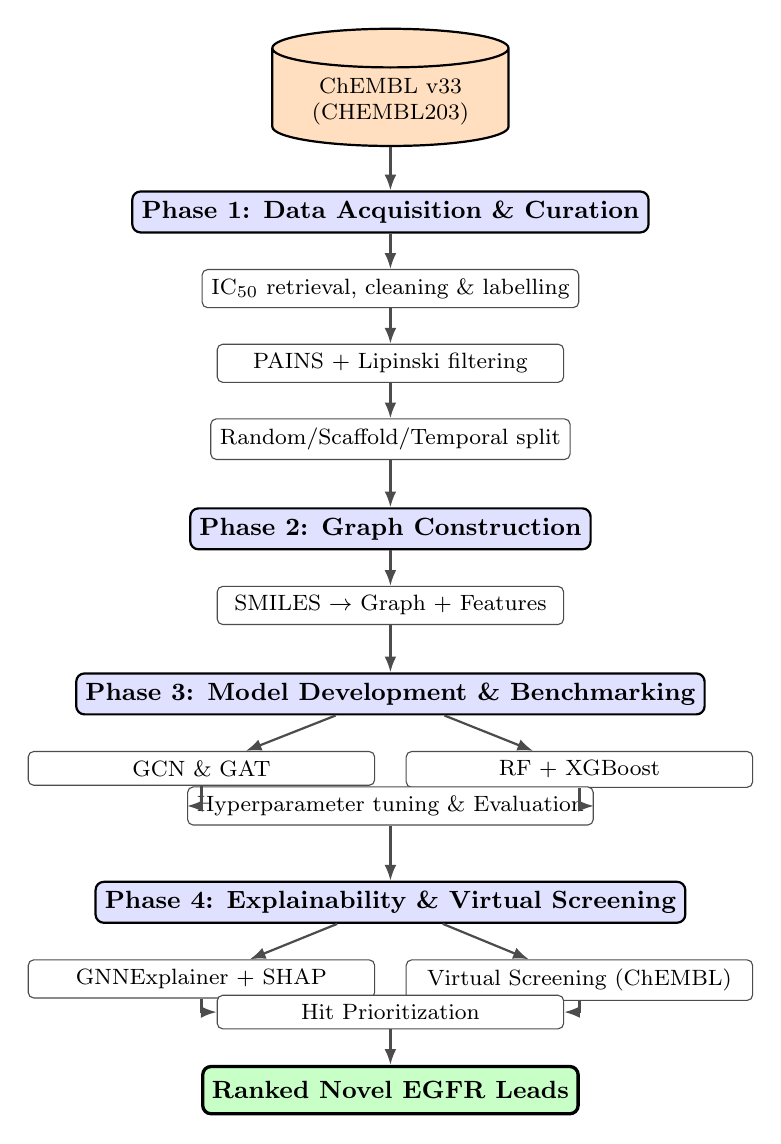
\begin{tikzpicture}[
    node distance=0.45cm and 0.35cm,
    font=\fontsize{8}{9.5}\selectfont,
    phase/.style={rectangle, rounded corners=3pt, draw=black, thick, minimum width=4.6cm, minimum height=0.52cm, fill=blue!12, align=center, font=\bfseries\small},
    process/.style={rectangle, rounded corners=2pt, draw=black!70, minimum width=4.4cm, minimum height=0.42cm, fill=white, align=center},
    data/.style={cylinder, shape border rotate=90, aspect=0.22, draw=black, thick, fill=orange!25, minimum width=3cm, minimum height=0.85cm, align=center},
    output/.style={rectangle, rounded corners=3pt, draw=black, very thick, minimum width=4.6cm, minimum height=0.6cm, fill=green!22, align=center, font=\small\bfseries},
    arrow/.style={-{Latex[length=2mm]}, thick, draw=black!70}
]

\node[data] (chembl) {ChEMBL v33\\(CHEMBL203)};

\node[phase, below=0.55cm of chembl] (p1) {Phase 1: Data Acquisition \& Curation};
\node[process, below=of p1] (p11) {IC$_{50}$ retrieval, cleaning \& labelling};
\node[process, below=of p11] (p12) {PAINS + Lipinski filtering};
\node[process, below=of p12] (p13) {Random/Scaffold/Temporal split};

\node[phase, below=0.6cm of p13] (p2) {Phase 2: Graph Construction};
\node[process, below=of p2] (p21) {SMILES $\to$ Graph + Features};

\node[phase, below=0.6cm of p21] (p3) {Phase 3: Model Development \& Benchmarking};
\node[process, below=of p3, xshift=-2.4cm] (gnn) {GCN \& GAT};
\node[process, below=of p3, xshift=2.4cm] (ml) {RF + XGBoost};
\node[process, below=0.9cm of p3] (tune) {Hyperparameter tuning \& Evaluation};

\node[phase, below=0.7cm of tune] (p4) {Phase 4: Explainability \& Virtual Screening};
\node[process, below=of p4, xshift=-2.4cm] (xai) {GNNExplainer + SHAP};
\node[process, below=of p4, xshift=2.4cm] (vs) {Virtual Screening (ChEMBL)};
\node[process, below=0.9cm of p4] (rank) {Hit Prioritization};

\node[output, below=of rank] (final) {Ranked Novel EGFR Leads};

\draw[arrow] (chembl) -- (p1);
\draw[arrow] (p1) -- (p11);
\draw[arrow] (p11) -- (p12);
\draw[arrow] (p12) -- (p13);
\draw[arrow] (p13) -- (p2);
\draw[arrow] (p2) -- (p21);
\draw[arrow] (p21) -- (p3);
\draw[arrow] (p3) -- (gnn);
\draw[arrow] (p3) -- (ml);
\draw[arrow] (gnn) |- (tune);
\draw[arrow] (ml)  |- (tune);
\draw[arrow] (tune) -- (p4);
\draw[arrow] (p4) -- (xai);
\draw[arrow] (p4) -- (vs);
\draw[arrow] (xai) |- (rank);
\draw[arrow] (vs)  |- (rank);
\draw[arrow] (rank) -- (final);

\end{tikzpicture}
\caption{Overall four-phase computational pipeline for EGFR inhibitor classification and lead identification.}
\label{fig:system-flow}
\end{figure}

\subsection{Phase 1: Data Acquisition and Curation}

\subsubsection{Data Source and Retrieval}

All bioactivity data for human EGFR (ChEMBL target: CHEMBL203) were retrieved from the ChEMBL database (version 33) using the \texttt{chembl\_webresource\_client} Python library with the following strict retrieval parameters: \texttt{standard\_type = `IC50'}, \texttt{standard\_units = `nM'}, \texttt{standard\_relation = `='}, and \texttt{assay\_type = `B'}.

\subsubsection{Data Cleaning}

\begin{itemize}
    \item \textbf{Missing value removal:} Entries with missing SMILES strings or IC$_{50}$ values were dropped.
    \item \textbf{Duplicate aggregation:} Compounds appearing multiple times were aggregated by taking the geometric mean of IC$_{50}$ values.
    \item \textbf{SMILES canonicalization:} All molecular structures were converted to canonical SMILES using RDKit, removing salts and solvents.
    \item \textbf{Structure validation:} Molecules that could not be parsed or sanitized by RDKit were discarded.
\end{itemize}

\subsubsection{Activity Labelling}

IC$_{50}$ values (in nM) were transformed to the pIC$_{50}$ scale:
\begin{equation}
    pIC_{50} = -\log_{10}\!\left(IC_{50} \times 10^{-9}\right)
\end{equation}

Binary activity labels were assigned using a threshold of $pIC_{50} \geq 6.0$ (equivalent to IC$_{50} \leq 1000$~nM): Active (Class~1) and Inactive (Class~0). This threshold is consistent with published EGFR cheminformatics practice \cite{malik2025}.

\subsubsection{Chemical Filtering}

\begin{itemize}
    \item \textbf{PAINS filtering:} Pan-Assay Interference Compounds were identified and removed using RDKit's \texttt{FilterCatalog} (PAINS\_A, PAINS\_B, PAINS\_C filters).
    \item \textbf{Lipinski's Rule of Five:} Compounds violating more than one criterion (MW $\leq 500$~Da, logP $\leq 5$, HBD $\leq 5$, HBA $\leq 10$) were removed.
\end{itemize}

\subsubsection{Data Splitting Strategies}

Three splitting strategies were employed:
\begin{itemize}
    \item \textbf{Random splitting (80/20):} Standard random train/test split, providing an upper-bound performance estimate.
    \item \textbf{Scaffold splitting (80/20):} Bemis--Murcko scaffold-based split using RDKit, evaluating generalisation to structurally novel scaffolds \cite{jiang2021}.
    \item \textbf{Temporal splitting:} Compounds split chronologically by ChEMBL assay date, evaluating prospective virtual screening performance.
\end{itemize}

\subsection{Phase 2: Molecular Graph Construction}

\subsubsection{Graph Representation}

Each curated molecule was converted from SMILES to a molecular graph $G = (V, E)$ using RDKit and PyTorch Geometric, where each node $v \in V$ represents one atom and each edge $e \in E$ represents one chemical bond.

\subsubsection{Node Features}

Each atom (node) was encoded as a 9-dimensional feature vector comprising the following properties. The \textbf{atomic number} encodes the element identity (C, N, O, F, S, etc.) as an integer. The \textbf{degree} records the number of covalently bonded neighbours as an integer. \textbf{Hybridization} is one-hot encoded across five states: sp, sp2, sp3, sp3d, and sp3d2. \textbf{Aromaticity} is a binary flag (0/1) indicating whether the atom belongs to an aromatic ring system. The \textbf{formal charge} encodes ionic state as a signed integer. The \textbf{hydrogen count} records the number of attached hydrogen atoms as an integer. \textbf{Ring membership} is a binary flag indicating whether the atom is part of any ring. \textbf{Chirality} (R/S stereochemistry) is one-hot encoded. Finally, \textbf{ring size} records the smallest ring size containing the atom as an integer. Together these nine features provide a compact yet chemically informative representation of each atom that captures both local electronic environment and topological context.

\subsubsection{Edge Features}

Each bond (edge) was encoded with four features: bond type (single, double, triple, aromatic; one-hot), conjugation status (binary), ring membership (binary), and stereochemistry E/Z type (one-hot).

\subsubsection{Exploratory Data Analysis}

Before model training, exploratory data analysis (EDA) was conducted: pIC$_{50}$ distributions and class balance were visualised using histograms; chemical space coverage was assessed by projecting Morgan fingerprints into 2D using t-SNE; and basic molecular property statistics were tabulated.

\subsection{Phase 3: GNN Model Development, Benchmarking, and Evaluation}

\subsubsection{GNN Architecture 1: Graph Convolutional Network (GCN)}

The primary GNN model is a three-layer GCN \cite{kipf2017}. In each layer, atom $i$ aggregates normalised features from all bonded neighbours and itself:
\begin{equation}
    h_i^{(l+1)} = \sigma \left( \sum_{j \in \mathcal{N}(i) \cup \{i\}} \frac{1}{\sqrt{\hat{d}_i \hat{d}_j}} \, W^{(l)} h_j^{(l)} \right)
\end{equation}

where $h_i^{(l)}$ is the embedding of atom $i$ at layer $l$; $\mathcal{N}(i)$ is the set of bonded atoms; $\hat{d}_i$ is the degree of atom $i$; $W^{(l)}$ is the learnable weight matrix; and $\sigma$ is the ReLU activation function. After three layers, global mean pooling produces a molecule-level embedding for binary classification.

\subsubsection{GNN Architecture 2: Graph Attention Network (GAT)}

The secondary model is a two-layer GAT \cite{velickovic2018}. GAT replaces fixed normalisation weights with learnable attention coefficients:
\begin{equation}
    \alpha_{ij} = \frac{\exp\!\left(\mathrm{LeakyReLU}\!\left( \mathbf{a}^T [W h_i \,\|\, W h_j] \right)\right)}{\sum_{k \in \mathcal{N}(i)} \exp\!\left(\mathrm{LeakyReLU}\!\left( \mathbf{a}^T [W h_i \,\|\, W h_k] \right)\right)}
\end{equation}

where $\mathbf{a}$ is a learnable attention vector and $\|$ denotes concatenation.

\subsubsection{Baseline Models}

Two traditional machine learning baselines were trained on Morgan fingerprints (ECFP4, radius = 2, 2048 bits):
\begin{itemize}
    \item \textbf{Random Forest (RF):} 200 trees, balanced class weights, maximum features = ``sqrt''.
    \item \textbf{XGBoost:} Learning rate = 0.05, max depth = 6, 300 estimators, subsample = 0.8.
\end{itemize}

\subsubsection{Hyperparameter Optimisation}

Key hyperparameters for both GCN and GAT models were tuned via grid search with 5-fold cross-validation on the scaffold-split training set. The \textbf{learning rate} was searched over \{0.0001, 0.001, 0.01\} and fixed at 0.001. The \textbf{hidden dimension} was evaluated at \{64, 128, 256\} and set to 128. The \textbf{number of GNN layers} was varied across \{2, 3, 4\} and fixed at 3. \textbf{Dropout rate} was searched over \{0.2, 0.3, 0.5\} and set to 0.3. \textbf{Batch size} was tested at \{32, 64, 128\} and fixed at 64. For the GAT model specifically, the \textbf{number of attention heads} was varied across \{2, 4, 8\} and fixed at 4. All models were trained for a maximum of 200 epochs with early stopping applied at a patience of 20 epochs to prevent overfitting.

\subsubsection{Training Configuration}

All GNN models were trained using the Adam optimiser with binary cross-entropy loss. 5-fold cross-validation was performed on the scaffold-split training set. Early stopping (patience = 20 epochs) was applied to prevent overfitting.

\subsubsection{Evaluation Metrics}

\begin{itemize}
    \item \textbf{AUC-ROC:} Area under the Receiver Operating Characteristic curve (1.0 = perfect; 0.5 = random).
    \item \textbf{Accuracy:} Fraction of correct predictions.
    \item \textbf{F1-Score:} Harmonic mean of precision and recall; appropriate for imbalanced datasets.
    \item \textbf{Matthews Correlation Coefficient (MCC):} Balanced metric considering all confusion matrix cells; the most informative single metric for imbalanced binary classification.
\end{itemize}

\subsection{Phase 4: Explainability Analysis and Virtual Screening}

\subsubsection{GNNExplainer: Instance-Level Molecular Explanation}

GNNExplainer \cite{ying2019} was applied via \texttt{torch\_geometric.explain.GNNExplainer} to the best-performing GNN model. For each molecule in the test set predicted as active, GNNExplainer identifies the minimal subgraph and node features maximising mutual information with the model's prediction:
\begin{equation}
    \max_{M, F} \; MI\!\left(Y,\, (G \odot M,\; X \odot F)\right)
\end{equation}
subject to sparsity constraints on edge mask $M$ and feature mask $F$. Results are visualised as colour-highlighted molecular graphs using RDKit's \texttt{Draw.MolToImage} function.

\subsubsection{SHAP: Global Feature Importance}

SHAP \cite{lundberg2017} was applied across the full test set to quantify which atomic node features most consistently drive predictions. The SHAP value for feature $i$ is:
\begin{equation}
    \phi_i = \sum_{S \subseteq F \setminus \{i\}} \frac{|S|!\,(|F|-|S|-1)!}{|F|!} \left[ f(S \cup \{i\}) - f(S) \right]
\end{equation}
SHAP summary bar plots and beeswarm plots were generated to show global feature importance rankings and the direction of each feature's effect.

\subsubsection{Chemical Interpretation}

GNNExplainer-identified substructures were compared to published EGFR pharmacophore models. RDKit substructure matching was used to quantify the frequency of highlighted fragments among active versus inactive compounds.

\subsubsection{Virtual Screening of Unseen ChEMBL Compounds}

The best-performing trained GNN model was applied to unseen compounds from ChEMBL (CHEMBL203) following a five-step workflow: (1) unseen compound preparation through the same curation pipeline; (2) Applicability Domain (AD) filtering using Tanimoto similarity $\geq 0.4$ \cite{tropsha2020}; (3) prediction and scoring with a high-confidence threshold of predicted active probability $\geq 0.80$; (4) hit prioritisation and ranking by predicted activity probability with structural novelty assessment; and (5) GNNExplainer visualisation of the top 10 ranked hits.

\subsection{Software and Tools}

All software used in this study is open-source. Python 3.10 served as the primary programming language. RDKit (2023.09+) was used for molecular processing, SMILES canonicalization, fingerprint computation, and graph construction. PyTorch (2.0+) provided the deep learning framework, and PyTorch Geometric (2.4+) provided GNN implementations and the GNNExplainer module. Scikit-learn (1.3+) was used for Random Forest, evaluation metrics, and scaffold splitting. XGBoost (2.0+) provided the gradient boosting baseline. SHAP (0.44+) was used for global feature importance analysis. Matplotlib (3.7+) and Seaborn (0.12+) were used for visualisation. Pandas (2.0+) and NumPy (1.24+) handled data processing. The \texttt{chembl-webresource-client} library was used for ChEMBL data retrieval, and JupyterLab (4.0+) provided the interactive development environment. The primary data source is the ChEMBL Database (version 33), target CHEMBL203, freely available at \url{https://www.ebi.ac.uk/chembl/}.

\newpage

% ==================== EXPECTED OUTCOMES ====================
\section*{Expected Outcomes}
\addcontentsline{toc}{section}{Expected Outcomes}

The expected outcomes of this study are directly aligned with the four specific objectives and four research questions stated in Chapter~1.

\begin{itemize}
    \item Fully trained and hyperparameter-optimised GCN and GAT models for binary EGFR inhibitor classification, with performance reported using AUC-ROC, accuracy, F1-score, and MCC under 5-fold cross-validation across all three splitting strategies (random, scaffold, and temporal).
    \item A comprehensive benchmarking table comparing GCN, GAT, Random Forest, and XGBoost, alongside a hyperparameter sensitivity analysis identifying which architectural choices most significantly impact GNN predictive performance.
    \item GNNExplainer atom-level and bond-level importance visualisations for representative active EGFR inhibitors from the test set; SHAP summary and beeswarm plots showing global atomic feature importance across the full dataset; and a written chemical interpretation comparing the identified substructures to known EGFR pharmacophore models from the medicinal chemistry literature.
    \item A ranked virtual screening hit list of potential novel EGFR inhibitor candidates from unseen ChEMBL (CHEMBL203) compounds, including predicted activity probability scores, structural novelty assessment via Tanimoto similarity to training set actives, and GNNExplainer visualisations for the top 10 highest-confidence hits.
    \item A fully reproducible open-source Python pipeline covering all four phases (data curation $\rightarrow$ graph construction $\rightarrow$ GNN training and benchmarking $\rightarrow$ explainability and virtual screening), suitable for adaptation to other kinase drug discovery targets, with potential for publication in a peer-reviewed journal of cheminformatics or computational medicinal chemistry.
\end{itemize}

\newpage

% ==================== WORK PLAN ====================
\section*{Work Plan of the Study}
\addcontentsline{toc}{section}{Work Plan of the Study}

The proposed time frame and activities of the study are presented below.

% §10.6(b): single spacing inside lengthy tables
\begin{table}[H]
\centering
{\singlespacing
\caption{Time Schedule}
\renewcommand{\arraystretch}{1.4}
\setlength{\tabcolsep}{4pt}
\begin{tabular}{|p{6.5cm}|*{4}{>{\centering\arraybackslash}p{0.9cm}|}}
\hline
\multirow{2}{*}{\textbf{Tasks}}
  & \multicolumn{4}{c|}{\textbf{Weeks}} \\
\cline{2-5}
  & \textbf{1} & \textbf{2} & \textbf{3} & \textbf{4} \\
\hline
Data acquisition and curation
  & \cellcolor{ganttblue} & & & \\
\hline
Feature engineering and EDA
  & \cellcolor{ganttblue} & \cellcolor{ganttblue} & & \\
\hline
Molecular graph construction
  & & \cellcolor{ganttblue} & & \\
\hline
Model development and evaluation
  & & \cellcolor{ganttblue} & \cellcolor{ganttblue} & \\
\hline
GNNExplainer and SHAP analysis
  & & & \cellcolor{ganttblue} & \\
\hline
Virtual screening
  & & & \cellcolor{ganttblue} & \cellcolor{ganttblue} \\
\hline
Hit prioritisation and validation
  & & & & \cellcolor{ganttblue} \\
\hline
Report writing and final submission
  & & & \cellcolor{ganttblue} & \cellcolor{ganttblue} \\
\hline
\end{tabular}
\label{tab:schedule}
}
\end{table}

\newpage

% ==================== REFERENCES ====================
% §10.6(b): References — single spacing within each entry,
% blank line spacing between entries
\section*{References and Citations}
\addcontentsline{toc}{section}{References}
{\singlespacing
\printbibliography
}
\end{document}